\documentclass[12pt]{article}
\usepackage[utf8]{inputenc}
\usepackage{enumerate}
\usepackage{amsmath}
\usepackage{amssymb}
\usepackage[margin=1.2in,footskip=0.25in]{geometry}
\usepackage{graphicx}
\usepackage{amsfonts}
\usepackage{array}
\usepackage{hyperref}

\hypersetup{
    colorlinks=true,
    linkcolor=blue,
    filecolor=magenta,      
    urlcolor=blue,
    pdftitle={Overleaf Example},
    pdfpagemode=FullScreen,
    }
%matriz ampliada
\newcommand{\uvec}[1]{\boldsymbol{\hat{\textbf{#1}}}}

\makeatletter
\renewcommand*\env@matrix[1][*\c@MaxMatrixCols c]{%
  \hskip -\arraycolsep
  \let\@ifnextchar\new@ifnextchar
  \array{#1}}
\makeatother

\AtBeginEnvironment{pmatrix}{\setlength{\arraycolsep}{5pt}}

%! TEX root = "~/home/ramiro/main.tex"
\setlength{\parindent}{0pt}
\title{\Huge{Title}}
\author{\huge{Ramiro Cabral}}
\date{\huge{}}

\begin{document}
\section{Archivos}
Los archivos poseen las siguientes caracteristicas:
\begin{itemize}
    \item Entidad abstractca con nombre.
    \item Espacio logico continuo y direccionable.
    \item Provee a los programas de datos (entrada).
    \item Permite a los programas guardar datos (salida).
    \item El programa mismo es informacin que debe guardarse.
\end{itemize}

\subsection{Objetivos del SO}
El SO busca cumplir con los siguientes objetivos en cuanto a archivos:
\begin{itemize}
    \item Cumplir con la gestion de datos.
    \item Cumplir con las solicitudes del usuario.
    \item Minimizar/eliminar la posibilidad de perder o destruir datos.
    \item Dar soporte de E/S a distintos dispositivos.
    \item Brindar un conjunto de interfaces de E/S para tratamiento de archivos.
\end{itemize}

\subsection{Derechos de Acesso}
Los derechos de acceso son los permisos que se le otorgan a los usuarios para que puedan acceder a los archivos.
Los derechos son los siguientes:
\begin{itemize}
    \item \textbf{Execution}: El usuario puede ejecutar.
    \item \textbf{Reading}: El usuario puede leer el archivo.
    \item \textbf{Appending}: El usuario puede agregar datos pero no modificar o borrar el contenido del archivo.
    \item \textbf{Updating}: El usuario puede modificar, borrar y agregar datos. Incluye la creacion de archivos, sobreescribirlo y remover datos.
    \item \textbf{Changing Protection}: El usuario puede modificar los derechos de acceso.
    \item \textbf{Owners(propietarios)}: Tiene todos los derechos, y pueden dar derechos a otros usuarios.
\end{itemize}


\section{Sistemas de Archivos}
Los sistemas de archivos son los encargados de organizar los archivos en el disco. Brindan espacio en disco a los archivos del usuario y del sistema, y mantienen un registro del espacio libre.
Algunos conceptos importantes son:
\begin{itemize}
    \item \textbf{Sector:} Unidad de almacenamiento utilizada en Discos Rigidos.
    \item \textbf{Cluster:} Conjuntos de sectores consecutivos.
    \item \textbf{File System:} Define la forma en que los datos son almacenados.
    \item \textbf{FAT (File Allocation Table:)} Contiene informacion sobre en que lugar estan alocados los distintos archivos.
\end{itemize}

\subsection{Asignacion de Espacio}

\subsubsection{Pre-Asignacion}
\begin{itemize}
    \item Se necesita saver cuanto espaci va a ocupar el archivo en el momento de su creacion.
    \item Se tiende a definir espacios mucho mas grandes que lo necesario.
    \item Posibilidad de utilizar sectores contiguos para almacenar los datos de un archivo.
\end{itemize}
\subsubsection{Asignacion Dinamica}
\begin{itemize}
    \item Se asigna espacio a medida que se va necesitando.
    \item Los bloques de datos pueden quedar de manera no contigua.
\end{itemize}

\subsubsection{Asignacion Continua}
\begin{itemize}
    \item Son utilizados conjuntos contiguos de bloques.
    \item Se requiere una pre-asignacion, es decir, conocer el tamaño del archivo durante la creacion.
    \item La FAT es simple: solo posee una entrada, que inclute el Bloque de Inicio y longitud.
    \item El archivo puede ser leido con una unica operacion.
    \item Puede existir fragmentacion externa, lo que se puede solucionar compactando el disco.
\end{itemize}
Posee distintos problemas, como por ejemplo el encontrar bloques libres continuos en el disco, y el hecho de que el tamaño del archivo aumente.
\vspace{2em}
\begin{figure}[h]
    \begin{center}
        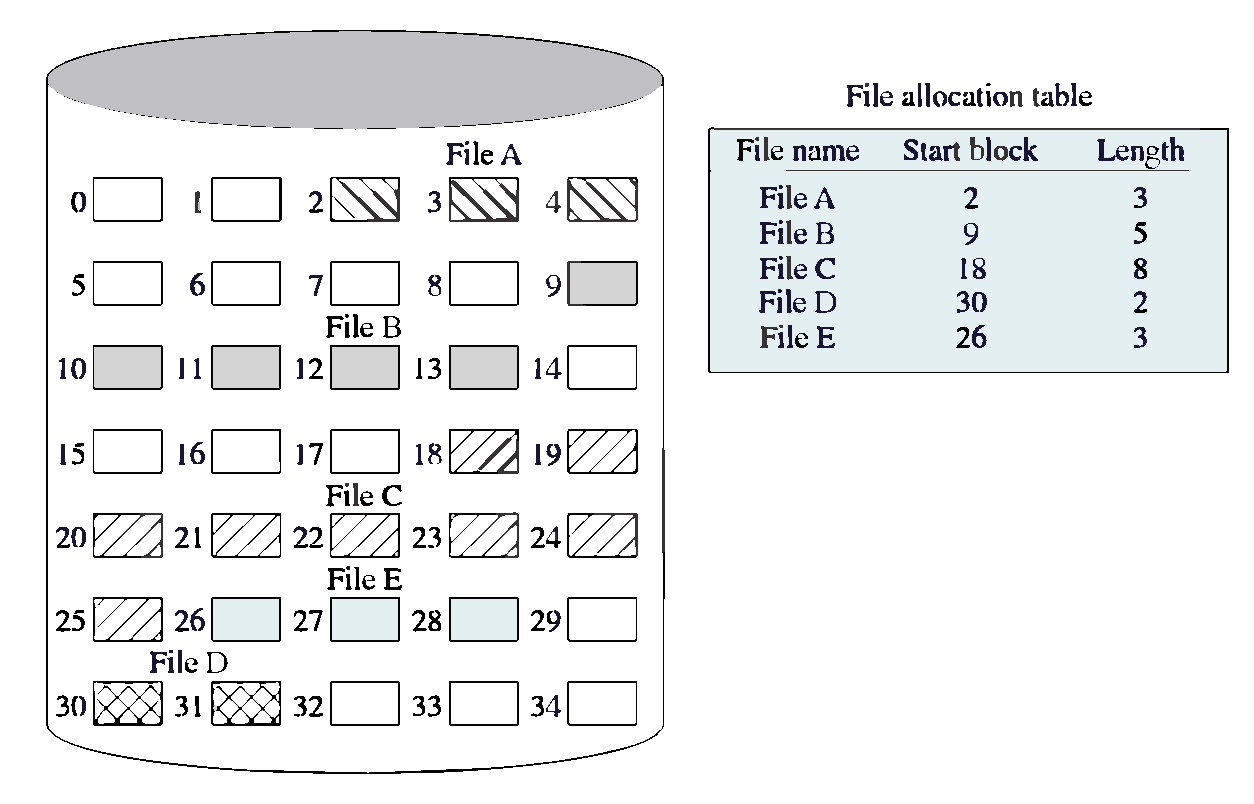
\includegraphics[width=0.85\textwidth]{assets/AsignacionContinua.pdf}
    \end{center}
    \caption{Asignacion Continua}
    \label{fig:3}
\end{figure}

\subsubsection{Asignacion Encadenada}
\begin{itemize}
    \item La asignacion se realiza en base a bloques individuales.
    \item Cada bloque tiene un puntero al proximo bloque del archivo.
    \item La FAT posee una unica entrada por archivo, el bloque de inicio y el tamaño del archivo.
    \item No hay fragmentacion externa.
    \item Es muy util para el acceso secuencial (no random).
    \item Los archivos pueden crecer bajo demanda, ya que no se requieren bloques contiguos.
    \item Se pueden consolidar los bloques de un mismo archivo para garantizar cercania de los bloques de un mismo archivo.
\end{itemize}


\begin{figure}[h]
    \begin{center}
        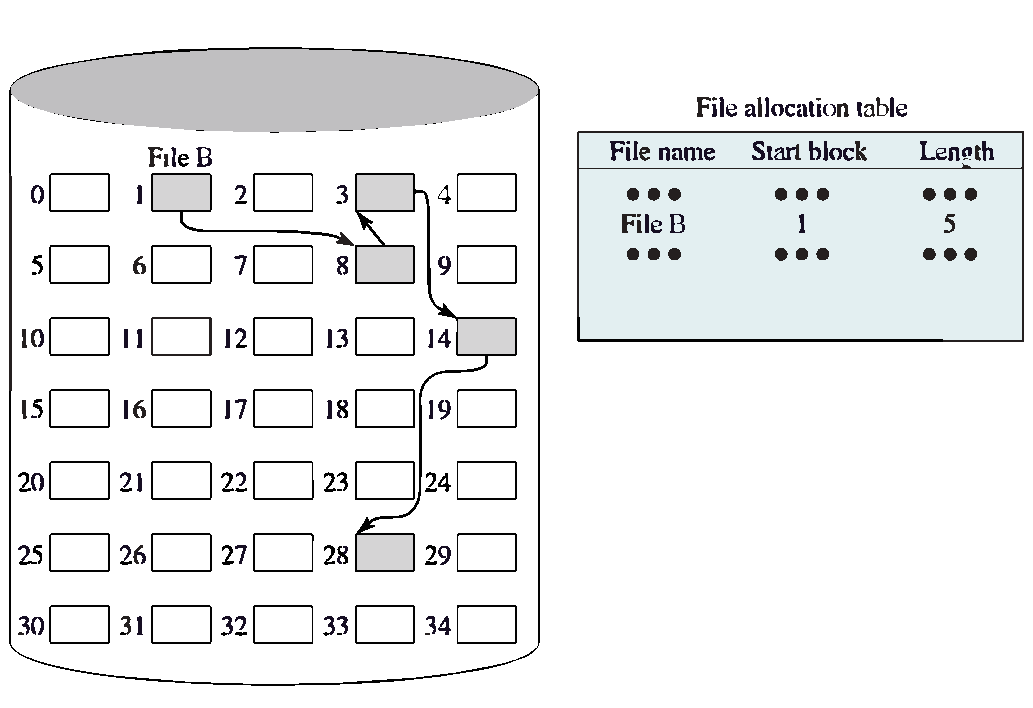
\includegraphics[width=0.80\textwidth]{assets/AsignacionEncadenada.pdf}
    \end{center}
    \caption{Asignacion Encadenada}
    \label{fig:4}
\end{figure}


\subsubsection{Asignacion Indexada}
\begin{itemize}
    \item La FAT contiene un punero al bloque indice.
    \item El bloque indice no contiene datos propios del archivo, sino que contiene un indice a los bloques que lo componen.
    \item La asignacion se realiza en base a bloques individuales.
    \item No produce fragmentacion externa.
    \item El acceso random a un archivo es eficiente.
    \item La FAT posee una unica entrada, con la direccion del bloque de indices (i-node).
\end{itemize}

\pagebreak

\begin{figure}[h]
    \begin{center}
        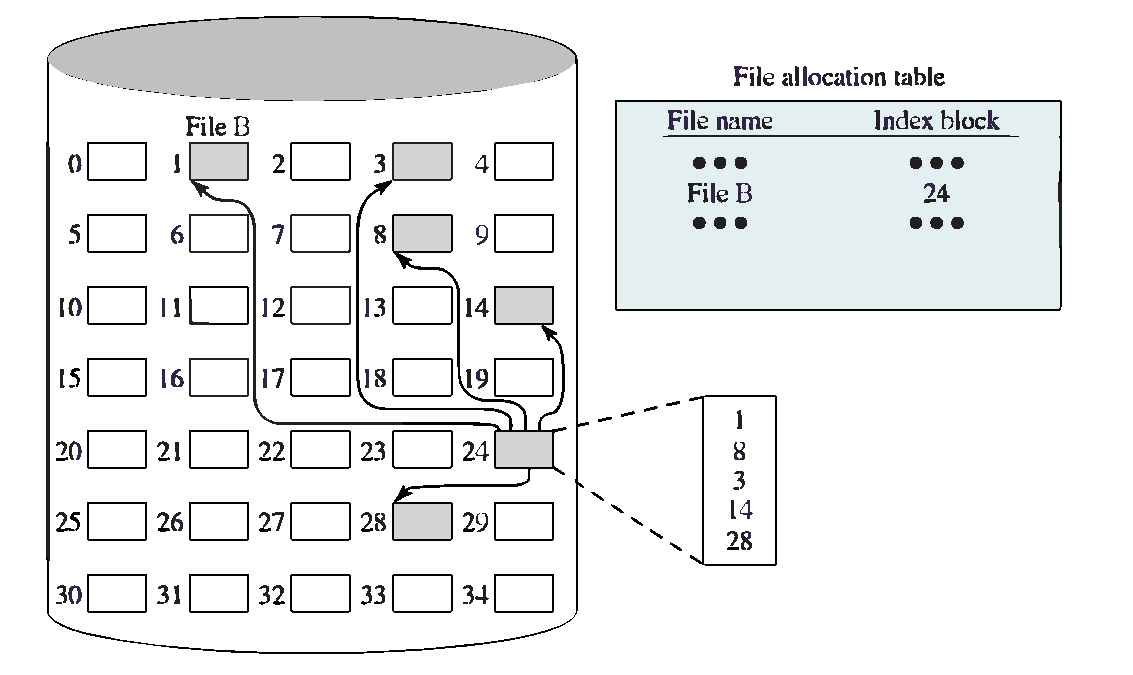
\includegraphics[width=0.75\textwidth]{assets/AsignacionIndexada.pdf}
    \end{center}
    \caption{Asignacion Indexada}
    \label{fig:5}
\end{figure}

\subsubsection{Asignacion Indexada - Variante por asignacion de secciones}
\begin{itemize}
    \item A cada entrada de bloque indice se agrega el campo longitud.
    \item El indice apunta al primer bloque de un conjunto almacenado de manera contigua.
\end{itemize}


\vspace{-8em}

\begin{figure}[ht]
    \begin{center}
        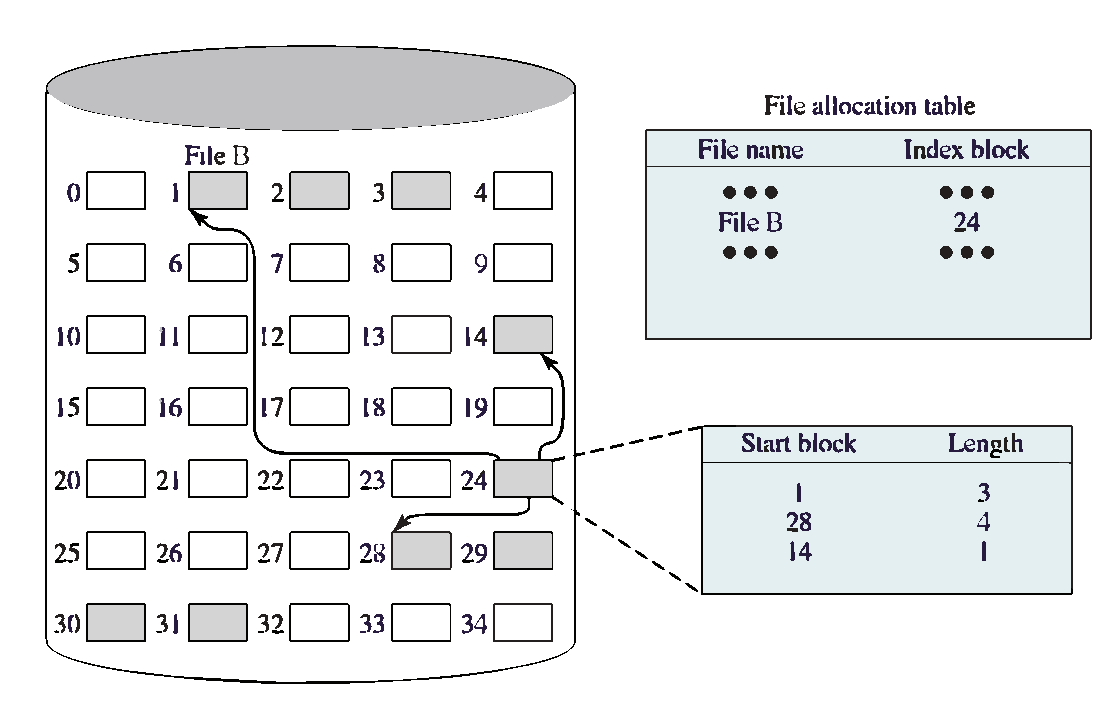
\includegraphics[width=0.75\textwidth]{assets/IndexadaSecciones.pdf}
    \end{center}
    \caption{Asignacion Indexada - Variante por asignacion de secciones}
    \label{fig:6}
\end{figure}

\pagebreak

\subsubsection{Asignacion Indexada - Variante por niveles de indireccion}
\begin{itemize}
    \item Existen bloques directos de datos.
    \item Otros bloques son considerados como bloque indices (apuntan a varios bloques de datos).
    \item Puede haber varios niveles de indireccion.
\end{itemize}

\begin{figure}[ht]
    \begin{center}
        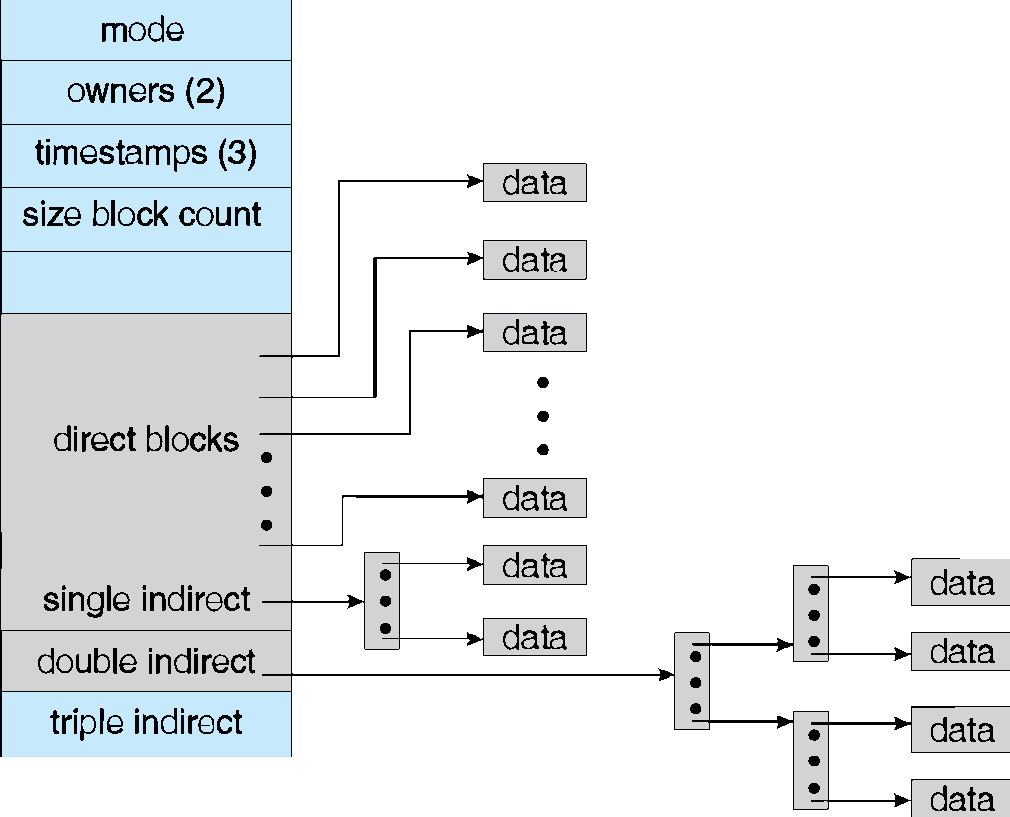
\includegraphics[width=0.70\textwidth]{assets/NivelesIndireccion.pdf}
    \end{center}
\end{figure}

\pagebreak

\subsection{Gestion de Espacio Libre}
Se necesita un control sobre cuales de los bloques de disco estan disponibles.

\subsubsection{Tabla de Bits}
\begin{itemize}
    \item Tabla (vector) con 1 bit por cada bloque de disco.
    \item Cada entrada: 0 = bloque libre, 1 = bloque ocupado.
    \item Es facil encontrar un bloque o grupo de bloques libres.
    \item El tamaño de la tabla es proporcional al tamaño del disco.
\end{itemize}

\subsubsection{Bloques Encadenados}
\begin{itemize}
    \item Se tiene un puntero al primer bloque libre.
    \item Cada bloque libre tiene un puntero al siguiente bloque libre.
    \item Ineficiente para la busqueda de bloques libres, ya que hay que realizar varias operaciones de I/O para obtener un grupo libre.
    \item Se producen problemas si se pierde un enlace.
\end{itemize}

\subsubsection{Indexacion o Agrupamiento}
\begin{itemize}
    \item Es una variante de los bloques libres encadenados.
    \item El primer bloque libre contiene las direcciones de N bloques libres.
    \item Las N-1 primeras direcciones son bloques libres.
    \item La N-esima direccion referencia otro bloque con N direcciones de bloques libres.
\end{itemize}

\end{document}
